\chapter{Other}


\begin{figure}
    \centering
    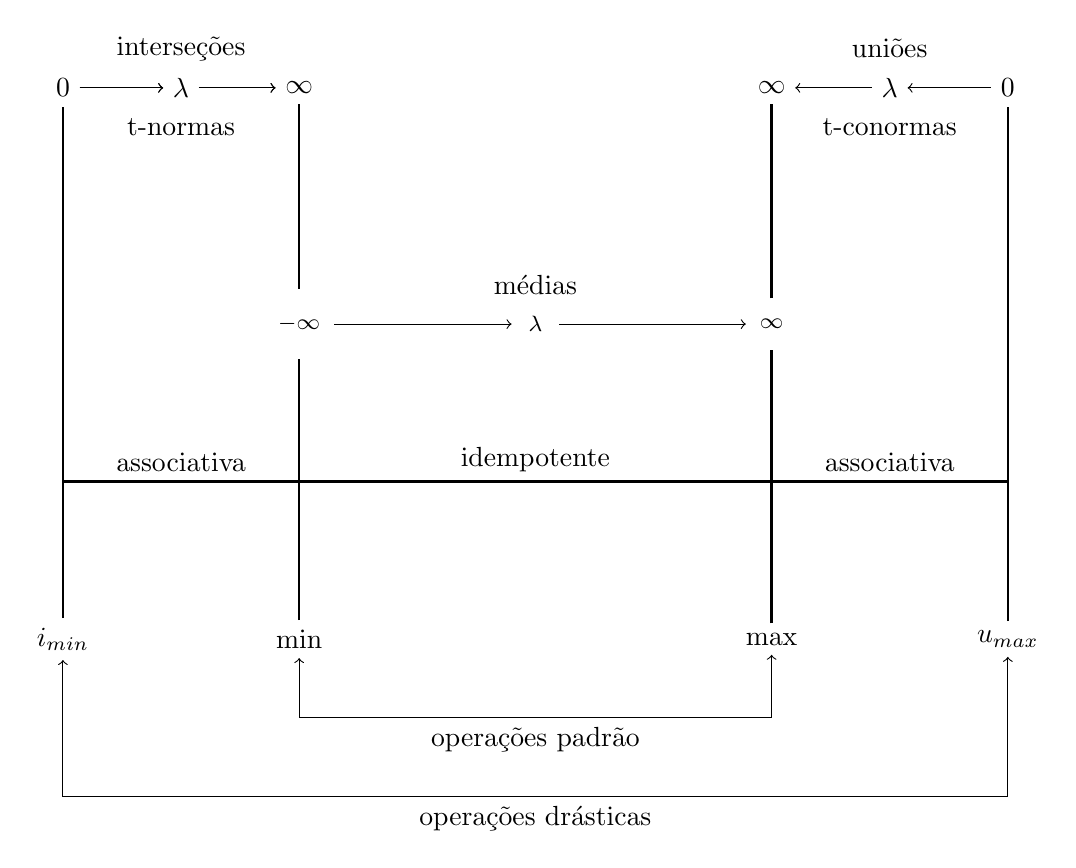
\begin{tikzpicture}
    [ bola/.style={circle,draw=white, fill=white,font=\footnotesize,text=black} ]
    
    \node (n1) at (0,10) {$0$} ;
    \node (n2) at (1.5,10) {$\lambda$};
    \node (n3) at (3,10) {$\infty$} ;  

    \draw[->] (n1.east) -- (n2.west);
    \draw[->] (n2.east) -- (n3.west);

    \node (n6) at (12,10) {$0$} ;
    \node (n5) at (10.5,10) {$\lambda$};
    \node (n4) at (9,10) {$\infty$} ;  
    
    \draw[<-] (n4.east) -- (n5.west);
    \draw[<-] (n5.east) -- (n6.west);
        
    \node (nimn) at  (0,3) {$i_{min}$};
    \node (numax) at (12,3) {$u_{max}$};
    \node (min) at (3,3) {$\min$};
    \node (max) at (9,3) {$\max$};
    \node at (1.5,10.5)  {interseções};
    \node at (1.5,9.5) {t-normas};
    \node at (10.5,10.5)  {uniões};
    \node at (10.5,9.5) {t-conormas};

    \draw[<->] (nimn.south) -- (0,1) -- (12,1)--(numax.south);
    \draw[<->] (min.south) -- (3,2) -- (9,2) --(max.south) ;

    \draw[->] (n1.east) -- (n2.west);
    \draw[->] (n2.east) -- (n3.west);


    \draw[thick] (0,5) -- (12,5);
    \node at (1.5,5) [above] {associativa};
    \node at (6,5) [above]   {idempotente};
    \node at (10.5,5) [above] {associativa};
    \node at (6,2) [below] {operações padrão};
    \node at (6,1) [below] {operações drásticas};
        
    \node (m1) at (3,7) [bola] {$-\infty$};
    \node (m2) at (6,7) [bola] {$\lambda$};
    \node (m3) at (9,7) [bola] {$\infty$};
    \draw[->] (m1.east) -- (m2.west);    
    \draw[->] (m2.east) -- (m3.west);    
    \node at (6,7.5) {médias};
    
    \draw[thick] (nimn.north) -- (n1.south);
    \draw[thick] (min.north) -- (m1.south) ;
    \draw[thick] (m1.north) -- (n3.south);
    \draw[thick] (max.north) -- (m3.south);
    \draw[thick] (m3.north) -- (n4.south);
    \draw[thick] (numax.north) -- (n6.south);

    \end{tikzpicture}
    \caption{Variáveis e posições}
  
\end{figure}



\begin{figure}[hbt]
\centering

\begin{tikzpicture}
 \draw[decorate,decoration={coil, aspect=0}] (0,0) circle (1.5cm);
\end{tikzpicture}
    \caption{Decorations need many libraries (at least)}
    
\end{figure}



\begin{figure}[hbt]
\centering
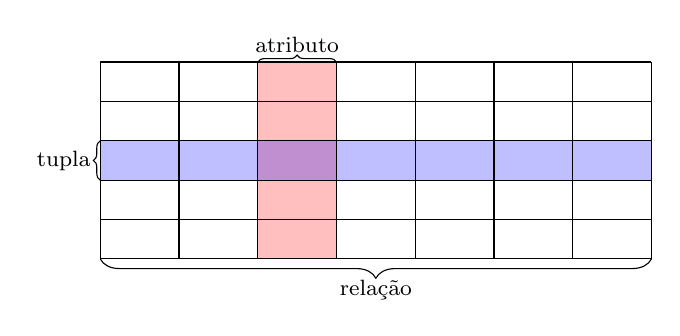
\begin{tikzpicture}
\fill[red,nearly transparent] (2,0) rectangle (3,2.5);
\fill[blue,nearly transparent] (0,1) rectangle (7,1.5);

\draw [decorate,decoration={brace}]
(2,2.5) -- (3,2.5)node [black,midway,above] {\footnotesize
 atributo };

\draw [decorate,decoration={brace}]
(0,1) -- (0,1.5)node [black,midway,left] {\footnotesize tupla};

\foreach \x in {0,1,2,3,4,5,6,7}
    \draw (\x,0) -- (\x,2.5);
\foreach \y in {0,.5,1,1.5,2,2.5}    
    \draw (0,\y) -- (7,\y);

\draw [decorate,decoration={brace,mirror,amplitude=7pt}]
(0,0) -- (7,0)node [black,midway,below=4pt] {\footnotesize{relação}};


\end{tikzpicture}


    \caption{Modelo abstrato de uma relação como uma tabela - usando decorations de chaves}

\end{figure}



\begin{figure}
\centering
\begin{tikzpicture}[description/.style={fill=white,inner sep=2pt},show background grid,show background rectangle]
    \useasboundingbox (-6.5,-5) rectangle (6.5,4);
    \scope[transform canvas={scale=.7}]
      \matrix (m) [matrix of math nodes, row sep=31pt,
    column sep=40pt, text height=1.5ex, text depth=0.25ex]
    { \\ \\ \\ \underset{v_0}{\bullet} & \underset{v_1}{\bullet} & \underset{v_2}{\bullet} & \underset{v_3}{\bullet} & \cdots & \underset{v_{\lambda - 3}}{\bullet} & \underset{v_{\lambda - 2}}{\bullet} & \underset{v_{\lambda - 1}}{\bullet} & \underset{v_\lambda}{\bullet} \\ \\ \\ \\ \\ \\ \\ \\ \underset{\hat v_0}{\bullet} & \underset{\hat v_1}{\bullet} & \underset{\hat v_2}{\bullet} & \underset{\hat v_3}{\bullet} & \cdots & \underset{\hat v_{\lambda - 3}}{\bullet} & \underset{\hat v_{\lambda - 2}}{\bullet} & \underset{\hat v_{\lambda - 1}}{\bullet} & \underset{\hat v_\lambda}{\bullet} \\};
    \path[->,font=\scriptsize]
    (m-4-1) edge [bend left=20] node[auto] {$1$} (m-4-2)
    (m-4-2) edge [bend left=20] node[auto] {$\lambda$} (m-4-1)
            edge [bend left=20] node[auto] {$2$} (m-4-3)
    (m-4-3) edge [bend left=20] node[auto] {$\lambda - 1$} (m-4-2)
            edge [bend left=20] node[auto] {$3$} (m-4-4)
    (m-4-4) edge [bend left=20] node[auto] {$\lambda - 2$} (m-4-3)
            edge [bend left=20] node[auto] {$4$} (m-4-5)
    (m-4-5) edge [bend left=20] node[auto] {$\lambda - 3$} (m-4-4)
            edge [bend left=20] node[auto] {$\lambda - 3$} (m-4-6)
    (m-4-6) edge [bend left=20] node[auto] {$4$} (m-4-5)
            edge [bend left=20] node[auto] {$\lambda - 2$} (m-4-7)
    (m-4-7) edge [bend left=20] node[auto] {$3$} (m-4-6)
            edge [bend left=20] node[auto] {$\lambda - 1$} (m-4-8)
    (m-4-8) edge [bend left=20] node[auto] {$2$} (m-4-7)
            edge [bend left=20] node[auto] {$\lambda$} (m-4-9)
    (m-4-9) edge [bend left=20] node[auto] {$1$} (m-4-8);
    \draw[<-] (m-4-1) .. controls +(70:50pt) and +(110:50pt) .. node[pos=.5, above]{\scriptsize $\lambda$} (m-4-1);
    \draw[<-] (m-4-2) .. controls +(70:50pt) and +(110:50pt) .. node[pos=.5, above]{\scriptsize $\lambda - 2$} (m-4-2);
    \draw[<-] (m-4-3) .. controls +(70:50pt) and +(110:50pt) .. node[pos=.5, above]{\scriptsize $\lambda - 4$} (m-4-3);
    \draw[<-] (m-4-4) .. controls +(70:50pt) and +(110:50pt) .. node[pos=.5, above]{\scriptsize $\lambda - 6$} (m-4-4);
    \draw[<-] (m-4-6) .. controls +(70:50pt) and +(110:50pt) .. node[pos=.5, above]{\scriptsize $6 - \lambda$} (m-4-6);
    \draw[<-] (m-4-7) .. controls +(70:50pt) and +(110:50pt) .. node[pos=.5, above]{\scriptsize $4 - \lambda$} (m-4-7);
    \draw[<-] (m-4-8) .. controls +(70:50pt) and +(110:50pt) .. node[pos=.5, above]{\scriptsize $2 - \lambda$} (m-4-8);
    \draw[<-] (m-4-9) .. controls +(70:50pt) and +(110:50pt) .. node[pos=.5, above]{\scriptsize $-\lambda$} (m-4-9);
    \path[draw] (-4.1, -2) rectangle (3.7, 0);
    \draw (-3.5, -1) node {$e$:};
    \draw[<-] (-3.2, -1) .. controls +(-20:18pt) and +(200:18pt) .. (-1.7, -1);
    \draw (-.5, -1) node {$f$:};
    \draw[->] (-.2, -1) .. controls +(20:18pt) and +(160:18pt) .. (1.3, -1);
    \draw (2.5, -1) node {$h$:};
    \draw[<-] (3.1, -1.5) .. controls +(70:40pt) and +(110:40pt) ..  (2.9, -1.5);
    \draw (-.5, 5) node {$V(\lambda)$};
    \path[->,font=\scriptsize]
    (m-12-1) edge [bend left=20] node[auto] {$\lambda$} (m-12-2)
    (m-12-2) edge [bend left=20] node[auto] {$1$} (m-12-1)
            edge [bend left=20] node[auto] {$\lambda - 1$} (m-12-3)
    (m-12-3) edge [bend left=20] node[auto] {$2$} (m-12-2)
            edge [bend left=20] node[auto] {$\lambda - 2$} (m-12-4)
    (m-12-4) edge [bend left=20] node[auto] {$3$} (m-12-3)
            edge [bend left=20] node[auto] {$\lambda - 3$} (m-12-5)
    (m-12-5) edge [bend left=20] node[auto] {$4$} (m-12-4)
            edge [bend left=20] node[auto] {$4$} (m-12-6)
    (m-12-6) edge [bend left=20] node[auto] {$\lambda - 3$} (m-12-5)
            edge [bend left=20] node[auto] {$3$} (m-12-7)
    (m-12-7) edge [bend left=20] node[auto] {$\lambda - 2$} (m-12-6)
            edge [bend left=20] node[auto] {$2$} (m-12-8)
    (m-12-8) edge [bend left=20] node[auto] {$\lambda - 1$} (m-12-7)
            edge [bend left=20] node[auto] {$1$} (m-12-9)
    (m-12-9) edge [bend left=20] node[auto] {$\lambda$} (m-12-8);
    \draw[<-] (m-12-1) .. controls +(70:50pt) and +(110:50pt) .. node[pos=.5, above]{\scriptsize $\lambda$} (m-12-1);
    \draw[<-] (m-12-2) .. controls +(70:50pt) and +(110:50pt) .. node[pos=.5, above]{\scriptsize $\lambda - 2$} (m-12-2);
    \draw[<-] (m-12-3) .. controls +(70:50pt) and +(110:50pt) .. node[pos=.5, above]{\scriptsize $\lambda - 4$} (m-12-3);
    \draw[<-] (m-12-4) .. controls +(70:50pt) and +(110:50pt) .. node[pos=.5, above]{\scriptsize $\lambda - 6$} (m-12-4);
    \draw[<-] (m-12-6) .. controls +(70:50pt) and +(110:50pt) .. node[pos=.5, above]{\scriptsize $6 - \lambda$} (m-12-6);
    \draw[<-] (m-12-7) .. controls +(70:50pt) and +(110:50pt) .. node[pos=.5, above]{\scriptsize $4 - \lambda$} (m-12-7);
    \draw[<-] (m-12-8) .. controls +(70:50pt) and +(110:50pt) .. node[pos=.5, above]{\scriptsize $2 - \lambda$} (m-12-8);
    \draw[<-] (m-12-9) .. controls +(70:50pt) and +(110:50pt) .. node[pos=.5, above]{\scriptsize $-\lambda$} (m-12-9);
    \draw (-.5, -4) node {$V(\lambda)^\ast$};
    \endscope
\end{tikzpicture}
\caption{
The manual states: “Tracking of the picture size is (locally) switched off …”
This means that the bounding box is lost, which needs to be specified manually via the useasboundingbox path (= path[use as bounding box]) which also needs to be outside of the scope that has transform canvas applied to.
You might consider the necessarity to transform your whole picture (this also affects font-sizes!).
} 
\end{figure}




\begin{figure}[hbt]
\centering
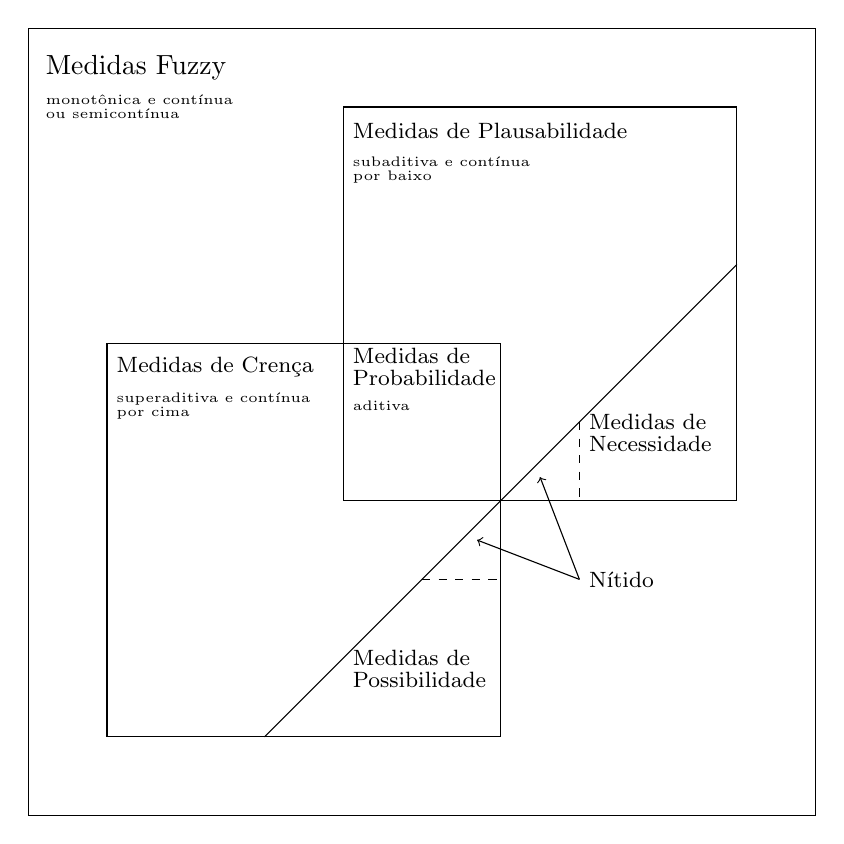
\begin{tikzpicture}

\draw  (0,0) rectangle (10,10) ;
\draw  (1,1) rectangle (6,6);
\draw  (4,4) rectangle (9,9);
\draw (3,1) -- (9,7) ;

\draw[dashed] (5,3) -- (6,3) ;
\draw[dashed] (7,5) -- (7,4) ;

\node at (0.1,9.5) [right] {Medidas Fuzzy};
\node at (0.1,9) [right,align=left,font=\fontsize{5pt}{5pt}\selectfont]
{monotônica e contínua \\ ou semicontínua};

\node at (4,5.7) [right,align=left,font=\fontsize{8pt}{8pt}\selectfont] 
{ Medidas de \\ Probabilidade};
\node at (4,5.2) [right,align=left,font=\fontsize{5pt}{5pt}\selectfont]
{aditiva};

\node at (1,5.7)
[right,align=left,font=\fontsize{8pt}{8pt}\selectfont] 
{Medidas de Crença};
\node at (1,5.2)
[right,align=left,font=\fontsize{5pt}{5pt}\selectfont]
{superaditiva e contínua \\ por cima };


\node at (4,8.7)
[right,align=left,font=\fontsize{8pt}{8pt}\selectfont]  
{Medidas de Plausabilidade};
\node at (4,8.2)
[right,align=left,font=\fontsize{5pt}{5pt}\selectfont]
{subaditiva e contínua \\ por baixo };

\node at (7,4.5)
[above right,align=left,font=\fontsize{8pt}{8pt}\selectfont]  
{Medidas de \\ Necessidade};

\node at (4,1.5)
[above right,align=left,font=\fontsize{8pt}{8pt}\selectfont]  
{Medidas de \\ Possibilidade};

\node at (7,3)
[right,align=left,font=\fontsize{8pt}{8pt}\selectfont] 
{Nítido};

\draw[->] (7,3) -- (6.5,4.3);
\draw[->] (7,3) -- (5.7,3.5);




\end{tikzpicture}


    \caption{Klir e os tipos de medida}
\end{figure}





















\begin{figure}
    \centering
\begin{tikzpicture}
\node[black,draw,rectangle,
    minimum width = 3cm, 
    minimum height = 4cm] (a) at (0,0) {$\gxmat{A'}$};
\node at (2cm,0) {$=$};
\node at (a.south) [below] {$t \times d$};
\node at (a.west) [left] {termos};
\node at (a.north) [above] {documentos};

\node[black,draw,rectangle,
    minimum width = 1cm, 
    minimum height = 4cm] (uu) at (3cm,0) {$\gxmat{U'}$};
\node[black,draw,rectangle,dashed,
    minimum width = 2cm, 
    minimum height = 4cm] (u) at (3.5cm,0) {};
\node at (uu.south) [below] {$d \times r$};    
\node at (5cm,0) {$\times$};


\node[black,draw,rectangle,
    minimum width = 1cm, 
    minimum height = 1cm] (ss) at (6cm,0.5) {};
\node[black,draw,rectangle,dashed,
    minimum width = 2cm, 
    minimum height = 2cm] (s) at (6.5cm,0) {};
\node at (ss.south) [below] {$r \times r$};
\node (sl) at (ss) {$\Sigma'$};
\draw[-] ($(ss.north west)+(0.1,-0.1)$) -- (sl.north west);
\draw[-] ($(ss.south east)+(-0.1,0.1)$) -- (sl.south east);

\node at (8cm,0) {$\times$}    ;


\node[black,draw,rectangle,
    minimum width = 3cm, 
    minimum height = 1cm] (vv) at (10cm,0.5) {};
\node[black,draw,rectangle,dashed,
    minimum width = 3cm, 
    minimum height = 2cm] (v) at (10cm,0) {};
\node (vl) at (vv) {$\gxmat{V}^T$};   
\node at (vv.south) [below] {$r \times d$};  
 \end{tikzpicture}
    \caption{LSI}
    \label{fig:lsi}
\end{figure}




\begin{figure}
    \centering
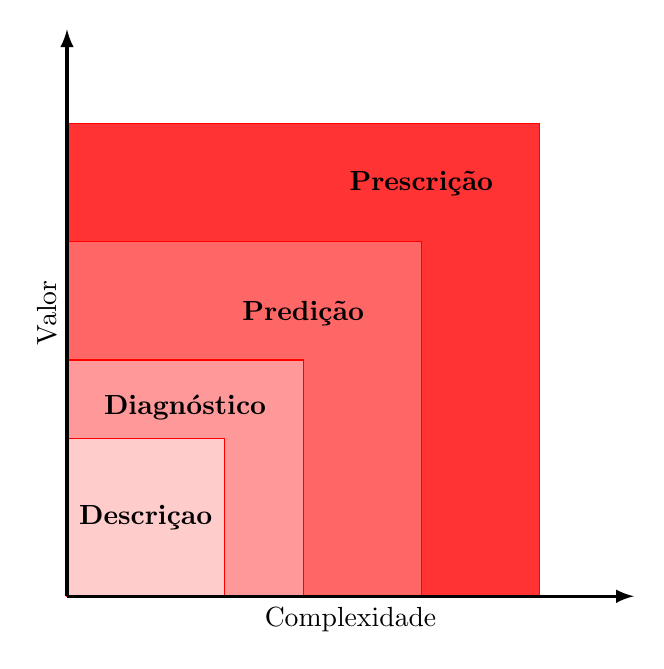
\begin{tikzpicture}
\tikzstyle{textbf} = [text centered,font=\bfseries]
\pgfmathsetmacro \s {6};
	\draw[red,fill = red!80] (0,0) rectangle (\s,\s);
	\draw[red,fill = red!60] (0,0) rectangle (\s*.75,\s*.75);
	\draw[red,fill = red!40] (0,0) rectangle (\s/2,\s/2);
	\draw[red,fill = red!20] (0,0) rectangle (\s/3,\s/3);
	\node[textbf] at (\s/6,\s/6) {Descriçao};
    \node[textbf] at (\s*.25,\s*.4) {Diagnóstico};
    \node[textbf] at (\s/2,\s*.6) {Predição};
    \node[textbf] at (\s*.75,\s/8*7)  {Prescrição};    
	\draw[very thick,-latex] (0,0) -> (\s*1.2,0)
	node [midway, below] {Complexidade};
	\draw[very thick,-latex] (0,0) -> (0,\s*1.2)
	node [midway, above ,rotate=90] {Valor};
\end{tikzpicture}
    \caption{Caption}
    \label{fig:my_labely}
\end{figure}

\begin{figure}
\centering
\begin{tikzpicture}

\filldraw[fill=green!40, draw=black,thick] (0,0.5) rectangle (4,6.5);
\filldraw[fill=red!40, draw=black,thick] (4,0.5) rectangle  (8,6.5);

\draw[fill=red,thick] (4,1.5) arc (-90:90:2cm);
\draw[fill=green,thick] (4,1.5) arc (-90:-270:2cm) -- (4,1.5);

\path (4,1.5) arc  (-90:-275:2cm) coordinate (A) ;

\node at (4,3) [above=.5cm,rotate=90,align=center] {$VP=A\cap B$ \\ relevantes \\ recuperados};
\node at (4,3) [above=.5cm,rotate=270,align=center] {$FP=B-A$ \\ não relevantes \\ recuperados};

\node at (2,6) [below,align=center] {$FN = A-B$} ;
\node at (6,6) [below,align=center] {$VN = C-A-B$};

\node at (2,0.5) [below,align=center] {relevantes \\ $A$ };
\node at (6,0.5) [below,align=center] {não relevantes \\ $C-A$};
\draw[-Latex] (4.3,6.6) node [above,align=center] {recuperados \\  $B$} -- (A) ;
\end{tikzpicture}
    \caption{Information Retrieval}
    \label{fig:my_label1}
\end{figure}






\begin{figure}
\centering
\begin{tikzpicture}[%
term/.style = {rounded corners = 6,%
minimum width = 6ex,%
minimum height = 4ex},%
every node/.style = {draw},%
every path/.style = {-latex},%
nd/.style = {minimum width = 10pt,%
minimum height = 36pt}]
\node[term] (t1) at (0,0) {T1};
\node[term,below = of t1] (t2) {T2};
\node[term,below = of t2] (t3) {T3};
\node[term,below = of t3] (t4) {T4};
\node[doc,nd, right = 3cm of t1] (d1) {D1};
\node[doc,nd, right = 3cm of t4] (d3) {D3};
\node[doc,nd] at ($(d1)!.5!(d3)$) (d2) {D2};
\draw (t1) -- (d1);
\draw (t2) -- (d1);
\draw (t3) -- (d1);
\draw (t3) -- (d2);
\draw (t3) -- (d3);
\draw (t4) -- (d3);
\end{tikzpicture}
\caption{Representação de um índice}
\end{figure}

\begin{figure}
\centering
\begin{tikzpicture}[%
term/.style = {rounded corners = 6,%
minimum width = 6ex,%
minimum height = 4ex},%
every node/.style = {draw},%
every path/.style = {-latex},%
nd/.style = {minimum width = 10pt,%
minimum height = 36pt}]
\node[term] (t1) at (0,0) {T1};
\node[term,below = of t1] (t2) {T2};
\node[term,below = of t2] (t3) {T3};
\node[term,below = of t3] (t4) {T4};
\node[cloud,right = of t2] (c1) {C1};
\node[cloud,right = of t3] (c2) {C2};
\node[doc,nd, right = 3cm of t1] (d1) {D1};
\node[doc,nd, right = 3cm of t4] (d3) {D3};
\node[doc,nd] at ($(d1)!.5!(d3)$) (d2) {D2};
\draw (t1) -- (c1);
\draw (t2) -- (c1);
\draw (t3) -- (c1);
\draw (t3) -- (c2);
\draw (t4) -- (c2);
\draw (c1) -- (d1);
\draw (c1) -- (d2);
\draw (c2) -- (d2);
\draw (c2) -- (d3);
\end{tikzpicture}
\caption{Representação do LSI/LSA}
\end{figure}



\begin{figure}
    \centering

\startchronology[startyear=1986,stopyear=2008,color=NavyBlue,dates=false]
\chronoperiode[color=lightgray,dates=false]{1986}{1991}{}
\setupchronoevent{colorbox=white}
\chronoevent{1986}{SGML}
\chronoevent{1991}{HTML}


\chronoevent[markdepth=-2cm]{1995}{JS}

\chronoevent[markdepth=1.5cm]{1996}{CSS}
\chronoevent[markdepth=2.5cm]{1999}{CSS 3}
\chronoevent[markdepth=1.5cm]{1998}{CSS 2}

\chronoevent{2005}{Ajax}
\chronoevent{2008}{HTML 5}

\chronoevent[markdepth=-1cm]{1996}{XML}

\chronoevent{1994}{HTML 2}
\chronoevent{1997}{HTML 4}
\chronoevent[markdepth=-1cm]{1991}{WWW}
\stopchronology

    \caption{Cronologia}
    \label{fig:my_labelx}
\end{figure}







\begin{figure}
\resizebox{\textwidth}{!}{
\begin{forest}
every path/.style={-latex}
[Métodos \\ de fusão \\ de termos,
for tree={align=center},for tree=draw,for tree=rounded corners=4,fill = yellow,for tree={minimum height=48pt,minimum width=6em,edge=-latex,anchor=center}
    [Manual]
    [Automático, fill = yellow
        [Termo\\Único,fill=yellow
            [Linguístico 
                [\textit{Finite-State}\\\textit{Transducer}]
            ]
            [Não \\ Linguístico, fill=yellow
                [Remoção \\de Afixos,fill=yellow
                    [Remoção \\ de Sufixos,fill=yellow
                        [Casamento \\ mais longo,fill=yellow]
                        [Remoção \\ Simples]
                    ]
                ]
                [Estatísticos
                    [n-gramas]
                    [HMM]
                    [Minial \\ Description \\ Length]
                    [Variedade de \\ Sucessores]
                ]
                [Busca em \\ Tabela]
                [Misto
                    [Flexões e \\ Derivaçoes]
                    [Baseados \\ em Corpus]
                ]
            ]
        ]
        [Termos\\com várias\\palavras
            [Não \\ Linguísticos \\ (Similaridade)
                [Co-ocorrência\\ de formas \\ de palavras]
                [Co-ocorrência \\ de n-gramas]
            ]
            [Linguísticos\\(Padrões \\\ Sintáticos)
                [\textit{Finite-State}\\\textit{Transducer}]
            ]
        ]
    ]
]
\end{forest}
}
\caption{Stemmers}

\end{figure}